\documentclass[11pt,twocolumn,oneside,openany,headings=optiontotoc,11pt,numbers=noenddot]{article}

\usepackage[a4paper]{geometry}
\usepackage[utf8]{inputenc}
\usepackage[T1]{fontenc}
\usepackage{lmodern}
\usepackage[ngerman]{babel}
\usepackage{ngerman}

\usepackage[onehalfspacing]{setspace}

\usepackage{fancyhdr}
\usepackage{fancybox}

\usepackage{rotating}
\usepackage{varwidth}

%Struktogramme
\usepackage[german,curves]{struktex}

\usepackage{pdflscape}
\usepackage{changepage}
\usepackage{graphicx}
\usepackage[bottom]{footmisc}
\usepackage{transparent}
\usepackage{graphbox}
\graphicspath{
	{Pics/PDFs/}
	{Pics/JPGs/}
	{Pics/PNGs/}
}
\usepackage{caption}
\usepackage{wrapfig}
\usepackage{marginnote}
\usepackage{tabularx}
\usepackage{dashrule}
\usepackage{soulutf8}
\usepackage{hhline}
%arydshln suppresses vertical lines in table
%\usepackage{arydshln}
\usepackage{multirow}
\usepackage{enumerate}
\usepackage[hidelinks]{hyperref}
\usepackage{listings}

\usepackage[table]{xcolor}
\usepackage{array}
\usepackage{enumitem,amssymb,amsmath}
\usepackage{interval}
\usepackage{cancel}
\usepackage{stmaryrd}
\usepackage{wasysym}
\usepackage{polynom}
\usepackage{diagbox}
\usepackage{dashrule}
\usepackage{framed}
\usepackage{mdframed}
\usepackage{karnaugh-map}
\usepackage{pdfpages}

\usepackage{blindtext}

\usepackage{eso-pic}

\usepackage{amssymb}
\usepackage{eurosym}

\usepackage[pages=some]{background}
\pagestyle{headings}
\renewcommand{\headrulewidth}{0.2pt}
\renewcommand{\footrulewidth}{0.2pt}
\newcommand*{\underdownarrow}[2]{\ensuremath{\underset{\overset{\Big\downarrow}{#2}}{#1}}}
\setlength{\fboxsep}{5pt}
\newcommand{\explainBelow}[3]{\underbrace{#1}_{\parbox{\widthof{#3}}{\footnotesize\raggedright #2}}}
\newcommand{\explainAbove}[3]{\overbrace{#1}^{\parbox{\widthof{#3}}{\footnotesize\raggedright #2}}}
\newcommand\footnoteref[1]{\protected@xdef\@thefnmark{\ref{#1}}\@footnotemark}


% Codestyle defined
\definecolor{codegreen}{rgb}{0,0.6,0}
\definecolor{codegray}{rgb}{0.5,0.5,0.5}
\definecolor{codepurple}{rgb}{0.58,0,0.82}
\definecolor{backcolour}{rgb}{0.95,0.95,0.92}
\definecolor{deepgreen}{rgb}{0,0.5,0}
\definecolor{darkblue}{rgb}{0,0,0.65}
\definecolor{mauve}{rgb}{0.40, 0.19,0.28}
\colorlet{exceptioncolour}{yellow!50!red}
\colorlet{commandcolour}{blue!60!black}
\colorlet{numpycolour}{blue!60!green}
\colorlet{specmethodcolour}{violet}

%Neue Spaltendefinition
\newcolumntype{L}[1]{>{\raggedright\let\newline\\\arraybackslash\hspace{0pt}}m{#1}}
\newcolumntype{M}{>{\centering\arraybackslash}X}
\newcommand{\cmnt}[1]{\ignorespaces}
%Textausrichtung ändern
\newcommand\tabrotate[1]{\rotatebox{90}{\raggedright#1\hspace{\tabcolsep}}}

%Intervall-Konfig
\intervalconfig {
	soft open fences
}

%Bash
\lstdefinestyle{BashInputStyle}{
	language=bash,
	basicstyle=\small\sffamily,
	backgroundcolor=\color{backcolour},
	columns=fullflexible,
	backgroundcolor=\color{backcolour},
	breaklines=true,
}
%Java
\lstdefinestyle{JavaInputStyle}{
	language=Java,
	backgroundcolor=\color{backcolour},
	aboveskip=1mm,
	belowskip=1mm,
	showstringspaces=false,
	columns=flexible,
	basicstyle={\footnotesize\ttfamily},
	numberstyle={\tiny},
	numbers=none,
	keywordstyle=\color{purple},,
	commentstyle=\color{deepgreen},
	stringstyle=\color{blue},
	emph={out},
	emphstyle=\color{darkblue},
	emph={[2]rand},
	emphstyle=[2]\color{specmethodcolour},
	breaklines=true,
	breakatwhitespace=true,
	tabsize=2,
}
%Python
\lstdefinestyle{PythonInputStyle}{
	language=Python,
	alsoletter={1234567890},
	aboveskip=1ex,
	basicstyle=\footnotesize,
	breaklines=true,
	breakatwhitespace= true,
	backgroundcolor=\color{backcolour},
	commentstyle=\color{red},
	otherkeywords={\ , \}, \{, \&,\|},
	emph={and,break,class,continue,def,yield,del,elif,else,%
		except,exec,finally,for,from,global,if,import,in,%
		lambda,not,or,pass,print,raise,return,try,while,assert},
	emphstyle=\color{exceptioncolour},
	emph={[2]True,False,None,min},
	emphstyle=[2]\color{specmethodcolour},
	emph={[3]object,type,isinstance,copy,deepcopy,zip,enumerate,reversed,list,len,dict,tuple,xrange,append,execfile,real,imag,reduce,str,repr},
	emphstyle=[3]\color{commandcolour},
	emph={[4]ode, fsolve, sqrt, exp, sin, cos, arccos, pi,  array, norm, solve, dot, arange, , isscalar, max, sum, flatten, shape, reshape, find, any, all, abs, plot, linspace, legend, quad, polyval,polyfit, hstack, concatenate,vstack,column_stack,empty,zeros,ones,rand,vander,grid,pcolor,eig,eigs,eigvals,svd,qr,tan,det,logspace,roll,mean,cumsum,cumprod,diff,vectorize,lstsq,cla,eye,xlabel,ylabel,squeeze},
	emphstyle=[4]\color{numpycolour},
	emph={[5]__init__,__add__,__mul__,__div__,__sub__,__call__,__getitem__,__setitem__,__eq__,__ne__,__nonzero__,__rmul__,__radd__,__repr__,__str__,__get__,__truediv__,__pow__,__name__,__future__,__all__},
	emphstyle=[5]\color{specmethodcolour},
	emph={[6]assert,range,yield},
	emphstyle=[6]\color{specmethodcolour}\bfseries,
	emph={[7]Exception,NameError,IndexError,SyntaxError,TypeError,ValueError,OverflowError,ZeroDivisionError,KeyboardInterrupt},
	emphstyle=[7]\color{specmethodcolour}\bfseries,
	emph={[8]taster,send,sendMail,capture,check,noMsg,go,move,switch,humTem,ventilate,buzz},
	emphstyle=[8]\color{blue},
	keywordstyle=\color{blue}\bfseries,
	rulecolor=\color{black!40},
	showstringspaces=false,
	stringstyle=\color{deepgreen}
}

\lstset{literate=%
	{Ö}{{\"O}}1
	{Ä}{{\"A}}1
	{Ü}{{\"U}}1
	{ß}{{\ss}}1
	{ü}{{\"u}}1
	{ä}{{\"a}}1
	{ö}{{\"o}}1
}

% Neue Klassenarbeits-Umgebung
\newenvironment{worksheet}[3]
% Begin-Bereich
{
	\newpage
	\sffamily
	\setcounter{page}{1}
	\ClearShipoutPicture
	\AddToShipoutPicture{
		\put(55,761){{
				\mbox{\parbox{385\unitlength}{\tiny \color{codegray}BBS I Mainz, #1 \newline #2
						\newline #3
					}
				}
			}
		}
		\put(455,761){{
				\mbox{\hspace{0.3cm}
\includegraphics[width=0.2\textwidth]{../../logo.pdf}}
			}
		}
	}
}
% End-Bereich
{
	\clearpage
	\ClearShipoutPicture
}

\setlength{\columnsep}{3em}
\setlength{\columnseprule}{0.5pt}

\geometry{left=2.50cm,right=2.50cm,top=3.00cm,bottom=1.00cm,includeheadfoot}
\pagenumbering{gobble}
\pagestyle{empty}

\begin{document}
	\begin{worksheet}{Höhere Berufsfachschule IT-Systeme}{Grundstufe - Mathematik}{Grundlagen}
		\begin{framed}
			Datum:
		\end{framed}
		\section{Allgemeine Begrifflichkeiten und Grundlagen}
		\subsection{Zahlen und Zahlenmengen}
		Aus dem Buch
		\subsection{Terme}
		\subsubsection*{Was sind Terme?} Unter einem Term versteht man ein \mbox{\textbf{mathematisches Gebilde}}. Dieses besteht aus Zahlen und Rechenzeichen.\\
		Eine Zahl kann hier aber auch durch einen Buchstaben angegeben werden.\\
		\par
		\begin{tabularx}{0.5\textwidth}{ll}
			\noindent
			\textbf{Beispiele:} & \(3\)\\
			& \(1,70+2,30\)\\
			& \(2,30\cdot x\)\\
			& \(5x + 20\)\\
			& \(5^2\)\\
			& \(\sqrt{5}\)\\
		\end{tabularx}
		\subsection{Termstrukturen}
		\paragraph{Warum sind sie wichtig?}
		Durch die Verwendung von Rechenzeichen innerhalb von Termen erhalten diese eine gewisse Struktur. In diversen Standardsituationen kann es sehr hilfreich sein, wenn man diese Strukturen erkennt.
		\begin{framed}
			\noindent
			\textbf{Beispiele:}\\
			\underline{Situation 1:} Berechnen von Funktionswerten:
			\[f(-3) = -2\cdot (-3)^2 + 4\]
			\textit{Welche Reihenfolge der Rechenoperationen muss beachtet werden? Tastenfolge im Taschenrechner?}\\
			\par\noindent
			\underline{Situation 2:} Lösen einer Gleichung mithilfe von Äquivalenzumformungen (z.B. zur Nullstellenbestimmung)
			\[-2x^2 +4 = 0\]
			\textit{Rechnet man zuerst }|\textit{\(:(-2)\), }|\textit{\(-4\) oder }|\textit{\glqq{}Wurzel\grqq{}?}
		\end{framed}
		\subsubsection*{Woraus bestehen diese?}
		Die Terme, mit denen Sie im Laufe der Zeit konfrontiert werden bestehen aus Summen, Produkten oder Potenzen.\\
		\par\noindent
		\textbf{\underline{Summen}}\\
		Eine \underline{Summe} besteht aus mindestens \textbf{zwei Summanden}, die durch ein \underline{\(+\)-Zeichen} verbunden sind.
		\begin{framed}\noindent
			\underline{Kurz:} Summand + Summand = Summe
		\end{framed}
		\noindent
		Führt man die Operation (Addition) aus, so erhält man den \underline{Summenwert}.\\
		\par\noindent
		\underline{Hinweis:} Sind zwei zahlen durch ein \underline{\glqq{}\(-\)\grqq{}-Zeichen} verbunden, spricht man von der \underline{Differenz}. Dieses Gebilde kann aber auch als Summe bezeichnet werden.\\
		\(7-4\) bedeutet nämlich eigentlich nichts anderes als \(7 + (-4)\). Es ist also eine Summe aus den Summanden \(7\) und \(-4\).\\
		\par\noindent
		\textbf{\underline{Produkte}}\\
		Ein \underline{Produkt} besteht aus mindestens \textbf{zwei Faktoren}. Diese werden durch ein \underline{\glqq{}\(\cdot\)\grqq{}-Zeichen} miteinander verbunden.
		\begin{framed}
			\noindent
			\underline{Kurz:} Faktor $\cdot$ Faktor = Produkt
		\end{framed}
		\noindent
		Führt man die Operation (Multiplikation) aus, erhält man den sogenannten \underline{Produktwert}.\\
		\par\noindent
		\underline{Hinweis:} Der Mal-Punkt wird häufig weggelassen. Also \(5\cdot x\) wird auch als \(5x\) geschrieben.\\
		\par\noindent
		\textbf{\underline{Potenzen}}\\
		Eine \underline{Potenz} besteht immer aus einer \textbf{Basis} und einem \textbf{Exponenten}. Dabei gibt der Exponent an, wie häufig die Basis mit sich selbst multipliziert wird.\\
		Führt man diese Rechnung aus, ergibt das den \underline{Potenzwert}.
		\begin{framed}
			\noindent
			\underline{Kurz:} \(Basis^{\text{Exponent}}\) = Potenz
		\end{framed}
		\noindent
		\underline{\textbf{Wurzel}}\\
		Die \underline{Wurzel} einer Zahl \(a\) bezeichnet die Zahl, die mit sich selbst multipliziert, den Wert \(a\) ergibt. In der Regel schreibt man \(\sqrt{a}\).\\
		Die Zahl unterhalb der Wurzel nennt man auch \textbf{Radikand}.
		\subsubsection{Wichtige Verknüpfungsregel}
		Es ist häufig der Fall, dass Potenzen, Produkte und Summern miteinander verknüpft werden. Ist dies der Fall, zerren unterschiedliche Rechenzeichen an einer Zahl herum.\\
		Bei der Berechnung des Werts eines Terms gilt die folgende Hierarchie:
		\begin{framed}
			\centering
			\color{red}Po\normalcolor{}tenzrechnung\\
			vor\\
			\color{red}Pu\normalcolor{}nktrechnung\\
			vor\\
			\color{red}Stri\normalcolor{}chrechnung!\\
			\normalcolor
			\par\noindent
			\raggedright
			Sind auch \color{red}Kla\normalcolor{}mmern beteiligt, so haben diese die größte Macht und binden am stärksten.
		\end{framed}
		\noindent
		\centering
		\fcolorbox{red!15}{red!5}{\textbf{\color{red}KlaPoPuStri}\normalcolor{} bewahrt vor Fehlern!}\\
		\raggedright
		\par\noindent
		\textbf{Beispiel 1:} \(4\cdot 2 + 5\)\\
		Wir analysieren die Termstruktur:
		\begin{tabularx}{0.5\textwidth}{c}
			\(4\ \boxed{\cdot}\ 2\ +\ 5\)\\
			\multicolumn{1}{l}{Zuerst \color{red}Pu\normalcolor{}nktrechnung:}\\
			\(=\ 8\ \boxed{+}\ 5\)\\
			\multicolumn{1}{l}{Dann \color{red}Stri\normalcolor{}chrechnung:}\\
			= 13
		\end{tabularx}
		\par\noindent
		\textbf{Beispiel 2:} \(4\cdot (2 + 5)\)\\
		Wir analysieren die Termstruktur:
		\begin{tabularx}{0.5\textwidth}{c}
			\(4\ \cdot\ \boxed{(}\ 2\ +\ 5\ \boxed{)}\)\\
			\multicolumn{1}{l}{Zuerst \color{red}Kla\normalcolor{}mmerausdruck auflösen:}\\
			\(=\ 4\ \boxed{\cdot}\ 7\)\\
			\multicolumn{1}{l}{Dann \color{red}Pu\normalcolor{}nktrechnung:}\\
			= 28
		\end{tabularx}
		\par\noindent
		\textbf{Beispiel 3:} \(-2\cdot{}(2+4)^2 + 7\)\\
		Wir analysieren die Termstruktur:
		\begin{tabularx}{0.5\textwidth}{c}
			\(-2\ \cdot{}\ \boxed{(}\ 2\ +\ 4\ \boxed{)}^2 +\ 7\)\\
			\multicolumn{1}{l}{Zuerst \color{red}Kla\normalcolor{}mmerausdruck auflösen:}\\
			\(=\ -2\ \cdot{}\ \boxed{6^2} +\ 7\)\\
			\multicolumn{1}{l}{Danach \color{red}Po\normalcolor{}tenz bestimmen:}\\
			\(=\ -2\ \boxed{\cdot{}}\ 36\ +\ 7\)\\
			\multicolumn{1}{l}{Anschließend \color{red}Kla\normalcolor{}mmerausdruck auflösen:}\\
			\(=\ -72\ \boxed{+}\ 7\)\\
			\multicolumn{1}{l}{Zuletzt \color{red}Stri\normalcolor{}chrechnung:}\\
			\(=\ -655\)\\
		\end{tabularx}
		\newpage
		\subsection{Rechenregeln}
		Ihnen ist sicher schon in den Sinn gekommen, dass Terme gegebenenfalls vereinfacht bzw. umgeformt werden können, um das Rechnen damit zu vereinfachen.
		\subsubsection*{Vorzeichenregel (VZ)}
		Für die Subtraktion und Addition negativer Zahlen gilt:
		\(-(-a) = +a\)\\
		\(+(-a) = -a\)\\
		\underline{Beispiel:} \(2 + (-3) = -1\)\\
		\par\noindent
		Für die Multiplikation von negativen Zahlen gilt:
		\((-)\cdot(-) = +\)\\
		\((+)\cdot(-) = +\)\\
		\((-)\cdot(+) = -\)\\
		\underline{Beispiel:} \((-2)\cdot(-4) = 8\)
		\subsubsection*{Klammerregeln - Ausmultiplizieren (AM)}
		Wird eine Summe als Klammerausdruck mit einer Zahl multipliziert, so muss jeder Summand aus der Klammer mit dieser Zahl multipliziert werden.\\
		\underline{Beispiel:} \(4\cdot(3+x) = 4\cdot{}3 + 4\cdot{}x = 12 + 4x\)
		\subsubsection*{Faktorisieren bzw. Ausklammern (FAK)}
		Bei einer Summe kann es durchaus passieren, dass alle Summanden einer Summe denselben Faktor enthalten. Diesen Faktor kann man dann ausklammern. Er wird also vor geschrieben. In die Klammer werden die Summe mit den verbleibenden Faktoren geschrieben.\\
		\par\noindent
		\underline{Beispiel:} Zwei Summanden: \(3x - 6\)\\
		Zunächst erkennen wir den gemeinsamen Faktor \((3)\).\\
		\(\mbox{3}x - \mbox{3}\cdot{}2\)\\
		Der Faktor wird zuerst aufgeschrieben, die übriggebliebenen Faktoren werden in der Klammer beibehalten.\\
		\(= \mbox{3}\cdot{}(x - 2)\)\\
		\par\noindent
		Es ergibt sich ein Produkt aus zwei Faktoren. Daher nennt man diese Operation auch \textbf{Faktorisieren}.\\
		\par\noindent
		Vielleicht haben Sie es bereits erkannt. \underline{Ausklammern ist die Umkehrung des Ausmul-} \underline{tiplizierens.}
		\begin{align*}
			\xrightarrow{\ Ausmultiplizieren}\\
			3(x-2) = 3x - 6\\
			\xleftarrow[\ \ \ Faktorisieren\ \ \ ]{}
		\end{align*}
		\subsubsection*{Minus vor der Klammer (MK)}
		Steht vor einem Klammerausdruck ein Minus (-), ist das nichts anderes als die Multiplikation der Klammer mit dem Wert \((-1)\).\\
		\underline{Beispiel:} \(-(2x + 2) = (-1)\cdot{}(2x+2) = -2x - 2\)\\
		Innerhalb einer Rechnung entspricht das dann:
		\begin{align*}
			& \ \ \ \ (2+a) - (3 - a)\\
			& = 2 + a + (-1)\cdot{}(3-a)\\
			& = 2 + a + (-1)\cdot{}3 + (-1)\cdot{}(-1)\\
			& = 2 + a - 3 + a\\
			& = -1 + 2a
		\end{align*}
		\subsubsection*{Binomische Formeln (BF)}
		Wird eine Summe/Differenz mit zwei Summanden bzw. Minuend und Subtrahend mit sich selbst multipliziert, kann man die binomische Formel anwenden:\\
		\begin{align*}
			\text{1. Binomische Formel}\\
			\mathbf{(a+b)^2} = (a + b)\cdot{}(a + b) & = \mathbf{a^2 + 2ab + b^2}\\
			\text{2. Binomische Formel}\\
			\mathbf{(a-b)^2} = (a - b)\cdot{}(a - b) & = \mathbf{a^2 - 2ab + b^2}\\
			\text{3. Binomische Formel}\\
			\mathbf{(a + b)\cdot{}(a - b)} & = \mathbf{a^2 - b^2}
		\end{align*}
		\underline{Beispiel:}
		\begin{align*}
			(x + 2)^2 & = x^2 + 2\cdot{}2\cdot{}x + 2^2\\
			& = x^2 + 4x + 4
		\end{align*}
		\subsubsection*{Zusammenfassen (ZUS)}
		Innerhalb einer Summe kann man Summanden zu einem Term zusammenfassen, sofern diese \glqq{}gleichartig\grqq{} sind.\\
		\underline{Beispiel:}\\
		\fcolorbox{red}{white}{\(x^2\)} \fcolorbox{blue}{white}{\(-\ 4x\)} \fcolorbox{green}{white}{\(+\ 3\)} \fcolorbox{blue}{white}{\(+\ 2x\)} \fcolorbox{green}{white}{\(-\ 4\)} \fcolorbox{red}{white}{\(+\ 2x^2\)}\\
		\par\noindent
		lässt sich wie folgt vereinfachen:\\
		\fcolorbox{white}{red!15}{\(3x^2\)} \fcolorbox{white}{blue!15}{\(-2x\)} \fcolorbox{white}{green!15}{\(-1\)}
		\subsubsection*{Potenzgesetze (PG)}
		Werden \underline{Potenzen} multipliziert oder dividiert, können auch diese \underline{zusammengefasst} werden. Dies ist aber nur dann möglich, wenn die \underline{Basis} oder der \underline{Exponent} gleich sind.\\
		Es gelten die folgenden Regeln:
		\begin{align*}
			a^m\cdot{}a^n & = a ^{m+n}\\
			\frac{a^m}{a^n} & = a^{m-n}\\
			a^m\cdot{}b^m & = (a\cdot{}b)^m\\
			\frac{a^m}{b^m} & = \left(\frac{a}{b}\right)^m\\
			(a^m)^n & = a^{m\cdot{}n}
		\end{align*}
		\newpage
		\underline{\textbf{Auch beim vereinfachen gilt} die Reihenfol-} \underline{ge von \color{red}KlaPoPuStri\normalcolor}. Also zuerst die Klammer vereinfachen, dann die Potenz, im Anschluss die Punktrechnung und abschließend die Strichrechnung!\\
		\par\bigskip\noindent
		\underline{\textbf{Beispiel:}} Versuchen sie den folgenden Term mit Hilfe der genannten Rechenregeln zu vereinfachen: \(2\cdot{}(x+2)^2 + 4x + 2\)
		\subsection{Brüche und Bruchterme}
		Buchtext
		%ToDo: Zu jedem Bereich Aufgaben
		\subsection{Ihre Aufgaben}
		\paragraph{(Zahlen und Zahlenmengen)} S.10 Nr. 1-3\\
		\paragraph{(Terme)} S.11 Nr. 1 und 2\\
		\paragraph{(Rechenregeln)} S.12 Nr. 1-3\\
		\paragraph{(Potenzen)} S. 15 Nr. 1 a-e / S. 15 Nr. 2 und 3\\
		\paragraph{(Brüche)} S. 13.Nr 1 und 2 / S. 14 Nr. 1-5 /\\
		\paragraph{(Wurzel)} S. 16 Nr 1-3\\
		\paragraph{(Gleichungen lösen)} S. 17 Nr. 1 und 2
		\paragraph{(Quadratische Gleichungen)} S. 19
		\paragraph{(Gleichungen der Form \((x-x_1)\cdot(x-x_2) = 0 \))}
		\newpage
		\section{Gleichungen und Ungleichungen}
		\subsection{Allgemeines zu Gleichungen und Ungleichungen}
		Sie wissen nun was ein Term ist. Es ist möglich zwei Terme mittels dem \glqq{}\(=\)\grqq{}-Zeichen miteinander zu verbinden. Ist dies der Fall, so liegt eine \underline{\textbf{Gleichung}} vor.\\
		\par\bigskip\noindent
		\underline{Beispiel:} \(18 + 0,5\cdot{}x = x\)\\
		\glqq{}\textit{Bei welcher Fahrtzeit macht es keinen Unterschied, ob man die Silber-Karte (18 \euro{} Grundgebühr und 0,50 \euro{} pro angefangene halbe Stunde) hat oder nicht (1 \euro{} pro angefangene Stunde)?}\grqq{}\\
		\par\bigskip\noindent
		Es besteht aber auch die Möglichkeit, zwei Terme mit einem \glqq{}\(<\)\grqq{} bzw. \glqq{}\(\leq\)\grqq{} (\glqq{}kleiner\grqq{} bzw. \glqq{}kleiner-gleich\grqq{}) oder \glqq{}\(>\)\grqq{} bzw. \glqq{}\(\geq\)\grqq{} (\glqq{}größer\grqq{} bzw. \glqq{}größer-gleich\grqq{}) zu verbinden.\\
		In diesem Fall handelt es sich um eine \underline{\textbf{Ungleichung}}.\\
		\par\bigskip\noindent
		\underline{Beispiel:} \(18 + 0,5x > 50\)\\
		\glqq{}\textit{Ab welcher Fahrtzeit übersteigen die Kosten einen Wert von 50 \euro{} pro Jahr?}\grqq{}\\
		\subsection{Die Lösungsmenge einer Gleichung}
		Gleichungen mit einer Variablen kann man lösen. Als Lösung einer Gleichung bezeichnet man die Zahlen als Besetzung der Variable, für die der Wert des rechten Terms gleich dem Wert des linken Terms ist.\\
		Alle Lösungen zusammen nennt man auch \underline{Lösungsmenge \(\mathbb{L}\)}.\\
		\par\bigskip\noindent
		\underline{Beispiel:} Die Lösungsmenge der Gleichung \(18 + 0,5x = x\) beträgt \(\mathbb{L} = {36}\) oder auch \(x=36\).
		\subsection{Die Lösungsmenge einer Gleichung bestimmen und angeben}
		Im Prinzip kann man sich eine Gleichung wie eine altmodische Waage vorstellen.\\
		
\includegraphics[width=0.1\textwidth]{../99_Bilder/waage.jpg} Dabei müssen die Gegenstände in den einzelnen Schalen nicht dieselbe Gestalt haben. Es ist aber unabdingbar, dass diese das gleiche Gewicht haben.\\
		\par\bigskip\noindent
		Ziel bei einer Waage ist es immer ein Gleichgewicht zu halten. Das bedeutet, führt man eine Operation auf der einen Seite durch, so muss diese auch auf der anderen Seite durchgeführt werden, damit das Gleichgewicht nicht gestört wird.\\
		Die Operationen kann man solange durchführen, bis man die Lösungsmenge erhält.\\
		\begin{framed}
			\noindent
			Im nachfolgenden Schauen wir uns ein Beispiel an.\\
			\centering
			
\includegraphics[width=0.4\textwidth]{../99_Bilder/L.jpg}\\
			\raggedright
			Wir entfernen nun zunächst einen Kreis und einen Kasten.\\
			\centering
			
\includegraphics[width=0.4\textwidth]{../99_Bilder/L1.jpg}\\
			\raggedright
			Es sind auf beiden Seiten eine gerade Anzahl an \glqq{}Gegenständen\grqq{}. Also halbieren wir diese.\\
			\centering
			
\includegraphics[width=0.4\textwidth]{../99_Bilder/L2.jpg}\\
			\raggedright
			Wir sehen also, ein Kasten entspricht zwei Kreisen.\\
		\end{framed}
		\par\bigskip\noindent
		Eine Gleichung immer mit der Waagendarstellung zu lösen kann sehr aufwendig sein. Man kann das Ganze auch symbolisch darstellen. Der Lösungsweg sieht dann so aus:
		\begin{tabularx}{0.5\textwidth}{rcll}
			\(3x + 1\) & \(=\) & \(x+5\) & |\(-1\)\\
			\(3x\) & \(=\) & \(x+4\) & |\(-x\)\\
			\(2x\) & \(=\) & \(4\) & |\(:2\)\\
			\(x\) & \(=\) & \(2\)
		\end{tabularx}
		Die Operationen, die man auf beiden Seiten der Gleichung durchführt, nennt man \underline{Äquivalenzumformung}. Die Umformungen sind so gewählt, dass die Termbestandteile mit \(x\) auf eine Seite und die Termbestandteile mit Zahlen auf die andere Seite gebracht werden.\\
		Man erhält also eine Gleichung der Form \(x = \text{Zahl}\).\\
		\par\bigskip\noindent
		Dabei ist \underline{zu beachten}, dass zunächst alle schwächsten Bindungen (\color{blue}Stri\normalcolor{}chrechnung) umgekehrt werden, danach die zweitschwächsten (\color{blue}Pu\normalcolor{}nktrechnung), dann die drittschwächsten (\color{blue}Po\normalcolor{}tenz) und zuletzt werden \color{blue}Kla\normalcolor{}mmern aufgelöst.\\
		\par\bigskip\noindent
		\centering
		\fcolorbox{blue}{blue!15}{\color{blue}StriPuPoKla\normalcolor{} löst die Gleichung!}\\
		\raggedright
		\par\bigskip\noindent
		Welche Operation welche Operation umkehrt ist nachfolgend aufgeführt:
		\begin{tabularx}{0.45\textwidth}{|c|c|X|}
			\cline{1-2}
			Operation & Umkehrung & \multicolumn{1}{l}{}\\
			\cline{1-2}
			\(+a\) & \(-a\) & \multicolumn{1}{l}{} \\
			\cline{1-2}
			\(-a\) & \(+a\) & \multicolumn{1}{l}{} \\
			\hline
			\multicolumn{1}{|l|}{} & & \\
			\(\cdot{}a\) & \(:a\) oder \(\cdot{}\frac{1}{a}\) &
			\multirow{7}{0.1\textheight}{Diese Operationen sind mit \textbf{allen Summanden auf beiden Seiten} durchzuführen!}\\
			\multicolumn{1}{|l|}{} & & \\
			\cline{1-2}
			\multicolumn{1}{|l|}{} & & \\
			\(:a\) oder \(\frac{\ldots}{a}\) & \(\cdot{}a\) & \\
			\multicolumn{1}{|l|}{} & & \\
			\cline{1-2}
			\multicolumn{1}{|l|}{} & & \\
			\(\ldots^2\) & \glqq{}\(\sqrt{\ldots}\)\grqq{} & \\
			\multicolumn{1}{|l|}{} & & \\
			\hline
		\end{tabularx}
		\par\bigskip\noindent
		\underline{Anmerkung zu \textbf{Äquivalenzumformung bei}} \underline{\textbf{Ungleichungen}:}\\
		Multipliziert oder dividiert man bei Ungleichungen mit einer negativen Zahl, dreht sich das Ungleichheitszeichen um.\\
		\underline{Beispiel:}
		\begin{tabularx}{0.5\textwidth}{cccl}
			\(-2x\) & \(<\) & \(4\) & |\(:(-2)\)\\
			\(x\) & \(>\) & \(-2\)
		\end{tabularx}
	\end{worksheet}
	\begin{worksheet}{Höhere Berufsfachschule IT-Systeme}{Grundstufe - Mathematik}{Grundlagen Funktionen}
		\setcounter{section}{0}
		\section{Begrifflichkeiten Funktionen}
		\subsection{Wertepaare} Häufig werden wir mit Wertepaaren (x-Wert, y-Wert) konfrontiert. Mehrere Wertepaare zusammengenommen können eine Entwicklung oder gewisse Abhängigkeiten darstellen.\\
		Diese können entweder in einer Tabelle oder als Punkte in Koordinatensystemen dargestellt werden.\\
		\par\bigskip\noindent
		\underline{Beispiel:} Wir betrachten zunächst einmal die Entwicklung der Instagram-Aktie im letzten Monat.\\
		Dabei gibt die \textbf{erste Komponente} des Wertepaares das Jahr an und die \textbf{zweite Komponente} den dazugehörigen Aktienkurs.\\
		\par\bigskip\noindent
		\begin{tabularx}{0.45\textwidth}{c|c}
			\textbf{Zeit} & \textbf{Kurs (in Euro)}\\
			(0 = 16.07.2018 & \\
			1 Einheit = 1 Tag) & \\
			\hline
			0 & 177,22\\
			\hline
			1 & 177,93\\
			\hline
			2 & 180,04\\
			\hline
			3 & 180,28\\
			\hline
			4 & 179,99\\
			\hline
		\end{tabularx}\\
		\par\noindent
		Als \underline{Punkte in einem Koordinatensystem} entspricht dies der nachfolgenden Darstellung:\\
		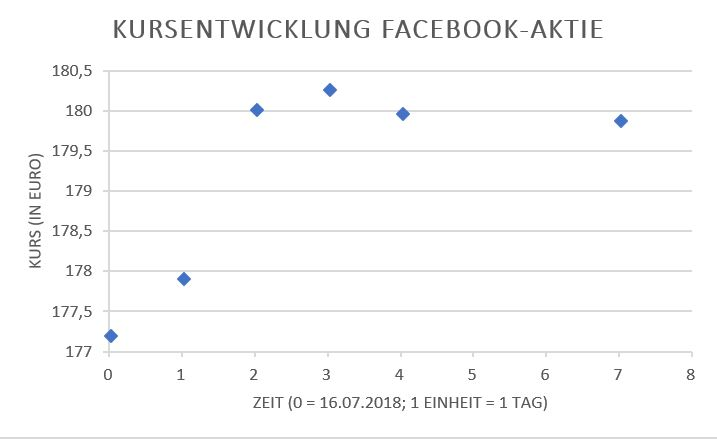
\includegraphics[width=0.45\textwidth]{../99_Bilder/fb.jpg}\\
		Ein weiteres \underline{Beispiel} kann der Lagerbestand von Bierkisten in einem Getränkemarkt sein.\\
		\par\bigskip\noindent
		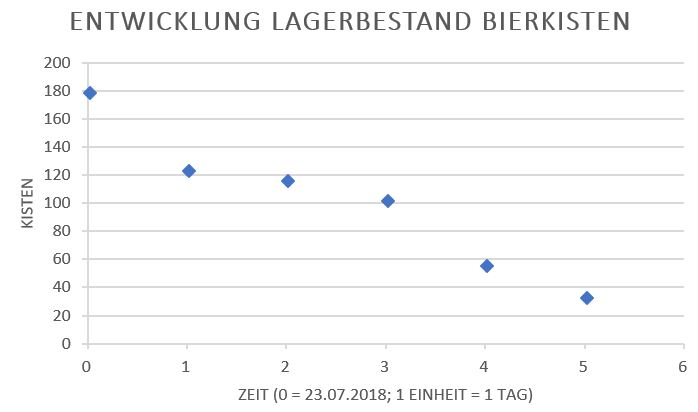
\includegraphics[width=0.5\textwidth]{../99_Bilder/bier.jpg}
		\subsection{Wertepaare werden zum Graphen}
		Wie im oberen Diagramm unschwer zu erkennen, können Punktdiagramme unübersichtlich sein. Abhilfe kann das Verbinden der einzelnen Punkte durch Linien schaffen.\\
		\par\bigskip\noindent
		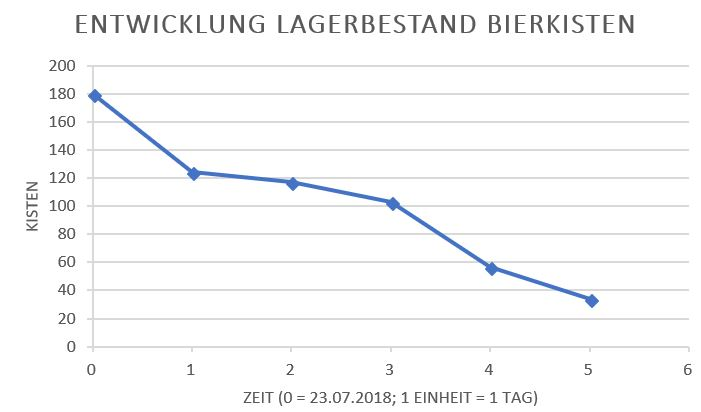
\includegraphics[width=0.5\textwidth]{../99_Bilder/bier1.jpg}\\
		\par\bigskip\noindent
		Für jede einzelne Verbindungslinie könnte man eine Entwicklung in einer Gleichung darstellen. Beim Lagerbestand wären das 5 verschiedene Gleichungen.\\
		Daher versucht eine glatte Trendlinie aufzustellen, so dass man die Entwicklung grob wiedergeben kann.\\
		\par\bigskip\noindent
		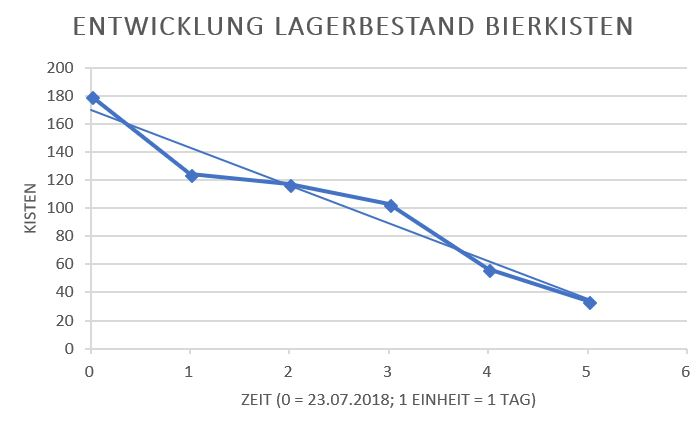
\includegraphics[width=0.5\textwidth]{../99_Bilder/bier2.jpg}\\
		\par\bigskip\noindent
		Diese Trendlinie kann durch die Gleichung
		\[y = -27x + 170\]
		angegeben werden.
		\subsection{Die Gleichung wird zum Graphen}
		Sind Sie mit der Aufgabe konfrontiert eine gegebene Gleichung in einem Koordinatensystem einzuzeichnen, ist der erste Schritt, entsprechende Wertepaare zu bestimmen. Dafür besetzt man das \(x\) der Gleichung mit einer Zahl und berechnet den Wert des Terms.\\
		Zur besseren Übersicht überträgt man diese Wertepaare in eine \textbf{\underline{Wertetabelle}}.\\
		\begin{tabularx}{0.45\textwidth}{|X|X|X|X|X|X|X|}
			\hline
			x & 0 & 1 & 2 & 3 & \(\ldots\) & \(\ldots\)\\
			\hline
			y & & & & & & \\
			\hline
		\end{tabularx}
		\subsubsection*{\underline{Ihre Aufgabe}} Berechnen Sie einige Wertepaare! Und übertragen diese in eine Wertetabelle.
		\begin{tabularx}{0.45\textwidth}{X}
			\(y = 4x + 12\)\\
			\(y = -3x - 21\)\\
			\(y = 2x - 5\)
		\end{tabularx}
		\par\bigskip\noindent
		Überträgt man die berechneten Wertepaare in ein Koordinatensystem und verbindet die einzelnen Punkte erhält man eine durchgezogene Linie. Diese repräsentiert im Prinzip nur die Aneinanderreihung von ganz vielen berechneten Wertepaaren.\\
		Diese durchgezogene Linie nennt man \underline{\textbf{Graph}}.
		\subsection{Modell vs. Realität}
		Wie Sie am Beispiel des Lagerbestands sicher bereits erkannt haben, gibt es Abweichungen zwischen dem realen Lagerbestand und der Trendlinie. Das ist darauf zurückzuführen, dass die Gleichung lediglich ein \underline{Modell} ist, das versucht, die Realität zu vereinfachen. Man kann sagen, dass ein Modell ein idealisiertes Abbild der Realität ist.\\
		\par\bigskip\noindent
		\begin{tabularx}{0.45\textwidth}{XX}
			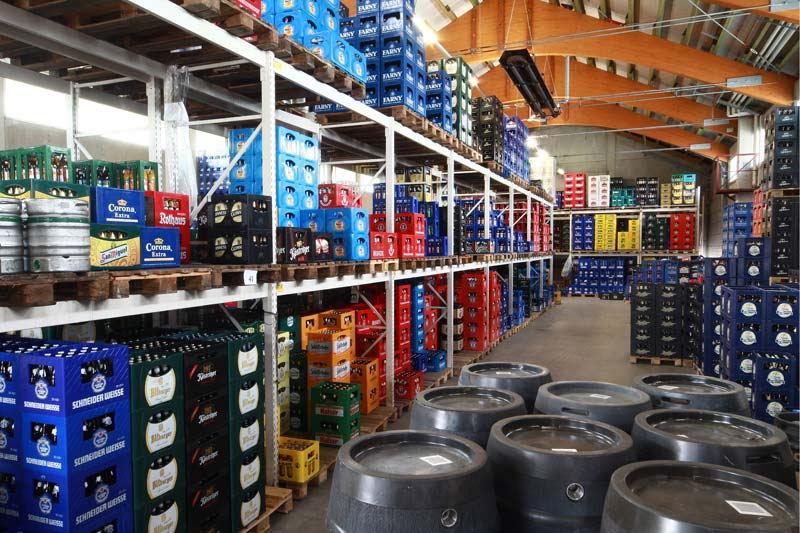
\includegraphics[width=0.25\textwidth]{../99_Bilder/lager.jpg} & 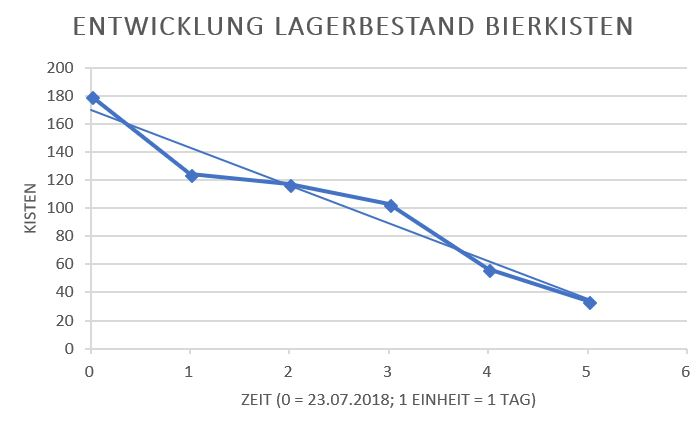
\includegraphics[width=0.25\textwidth]{../99_Bilder/bier2.jpg}
		\end{tabularx}
		\par\bigskip\noindent
		\underline{Vorteile des Modells:}
		\begin{itemize}
			\item[-] geradliniger Graph ohne Zacken
			\item[-] Analyse der Entwicklung möglich
			\item[-] Darstellung der Entwicklung mittels einer Gleichung
			\item[-] Fortführung des Modells möglich (Prognose)
		\end{itemize}
		Ein Modell hat aber nicht nur Vorteile. Ein wesentlicher \underline{Nachteil des Modells} ist, dass der Informationsgehalt eingeschränkt ist, da Ausschläge und Abweichungen einfach weggelassen werden.
		\newpage
		\section{Der Begriff \glqq{}Funktion\grqq{}}
		\begin{framed}
			\noindent
			\paragraph{Definition:} Eine Funktion entspricht einer Menge von Wertepaaren, welche aus zwei Mengen gebildet wird. Jedem Element der Ausgangsmenge (Definitionsmenge oder auch \(\mathbb{D}\)) wird ein Element der Zielmenge (Wertemenge oder auch \(\mathbb{W}\)) zugeordnet.
		\end{framed}
		\noindent
		Nimmt man zum Beispiel das Element \(x=4\) aus \(\mathbb{D}\), so gibt einem die Funktion den entsprechenden Lagerstand zu diesem Zeitpunkt. So ergibt sich das Wertepaar \((4|62)\).\\
		\par\bigskip\noindent
		Das Element der Ausgangsmenge bezeichnet man als \underline{\textbf{x-Koordinate}} und das Element der Wertemenge nennt sich \underline{\textbf{y-Koordinate}}.\\
		\par\bigskip\noindent
		Im Prinzip ist also eine Funktion nichts anderes als eine Menge von Wertepaaren, die aus einer bestimmten Vorschrift (der Funktion) hervorgehen. Daher kann man mit Hilfe von Funktionen Entwicklungen und Abhängigkeiten beschreiben oder modellieren.
		\subsection{Darstellungsformen von Funktionen}
		Eine Funktion kann auf verschiedene Arten dargestellt werden.
		\subsubsection*{Funktionsterm und Funktionsgleichung}
		Der Funktionsterm gibt die Anweisung zur Erzeugung der Wertepaare. Diese entstehen dadurch, dass man die Variable durch eine Zahl (erste Komponente) besetzt und den Wert des Terms (zweite Komponente) berechnet.\\
		Als Funktionsgleichung hingegen bezeichnet man den Ausdruck, dem Term \(y\) den Funktionsterm durch das \glqq{}\(=\)\grqq{}-Zeichen zuweist.\\
		\par\bigskip\noindent
		\begin{align*}
			\underbrace{y = \overbrace{200 -18x}^{\text{Funktionsterm}}}_{\text{Funktionsgleichung}}
		\end{align*}
		\subsubsection*{Wertetabelle}
		Hat man hingegen Wertepaare gebildet, kann man diese in einer Wertetabelle festhalten. Diese spiegeln eindeutig die Funktion wider.\\
		\par\bigskip\noindent
		\begin{tabularx}{0.5\textwidth}{|X|l|l|l|l|l|l|}
			\hline
			x & 0 & 1 & 2 & 3 & 4 & 5\\
			\hline
			\(y = -27x + 170\) & 170 & 143 & 116 & 89 & 62 & 35\\
			\hline
		\end{tabularx}
		\subsubsection*{Graph}
		Hat man Wertepaare gegeben, kann man diese als Punkte in ein Koordinatensystem übertragen.\\
		\underline{Anmerkung zur Skalierung:} Man erkennt, dass der Bestand Werte zwischen 170 und 35 annimmt. Daher sollten die Einheit für die y-Achse 17 haben \((170:10 = 17)\)\\
		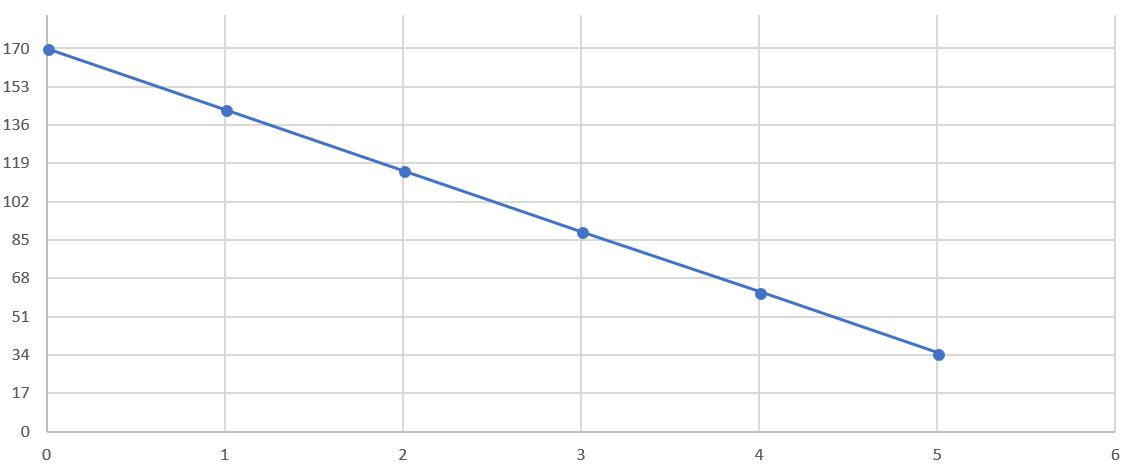
\includegraphics[width=0.45\textwidth]{../99_Bilder/bierkoord.jpg}\\
		\par\bigskip\noindent
		Die Menge der Punkte, die durch das Verbinden der einzelnen Wertepaar-Punkte entsteht nennt man auch \underline{\textbf{Graph der Funktion}}. Häufig ist es aber nur möglich einen bestimmten Abschnitt des \underline{Funktionsgraphen} zu zeichnen.\\
		\par\bigskip\noindent
		Genaugenommen ist es uns nicht möglich einen Punkt oder den Graph einer Funktion zu zeichnen. Das oben dargestellt ist lediglich der intuitiven Anwendung unserer Erfahrung geschuldet.\\
		Das Verbinden der Punkte mit dem Lineal ist nur bei \textbf{linearen Funktionen} möglich.\\
		\textit{\color{red}{Im Allgemeinen gilt: Das Verwenden des Lineals zum Verbinden der Punkte ist streng verboten!}}\\
		\subsubsection*{\underline{Ihre Aufgabe}}
		Zeichnen Sie einen sauberen Graphen für die Funktionsgleichung \(\mathbf{y = 200-18x}\).\\
		Nutzen Sie dafür eine Wertetabelle.
		\section{Begriffe zur Beschreibung eines Graphen}
		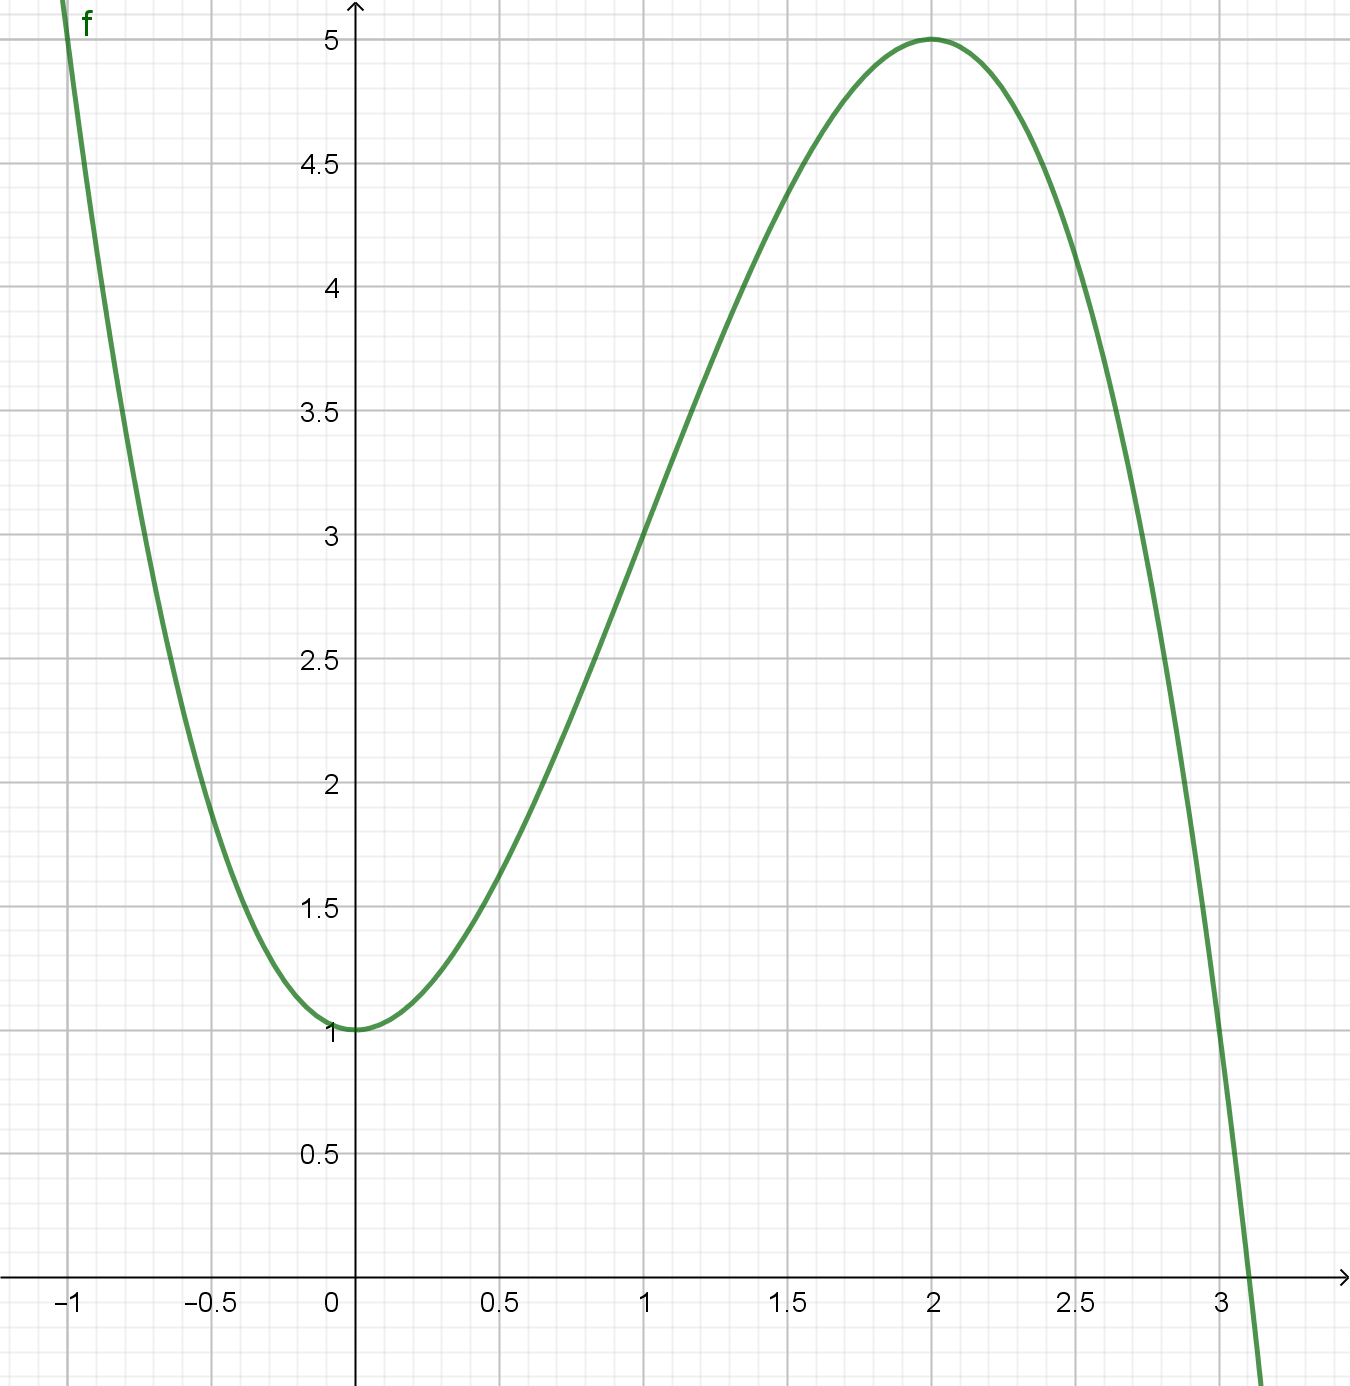
\includegraphics[width=0.49\textwidth]{../99_Bilder/basicsBsp.png}\\
		\par\bigskip\noindent
		Stellen Sie sich vor, Sie müssten den oben dargestellten Graphen am Telefon beschreiben. Welche Charakteristika würden Sie nennen?
		\subsection*{y-Achsenabschnittswert}
		Der Wert, bei dem der Graph die y-Achse schneidet, nennt man \textbf{\underline{y-Achsenabschnitt}}. Rechnerisch erhält man diesen Wert dadurch, dass man \(x= 0\) besetzt.\\
		\par\bigskip\noindent
		\textbf{Wichtig: Die y-Achse hat \underline{Werte}.}
		\subsection*{Nullstelle(n)}
		Die Stellen, an denen der Graph die x-Achse schneidet, nennt man \textbf{\underline{Nullstellen}}. Um diese Nullstellen zu berechnen, löst man die Gleichung \(y = 0\).\\
		\par\bigskip\noindent
		\textbf{Achtung: Auf der x-Achse gibt es nur \underline{Stellen}.}\\
		\includegraphics[width=0.49\textwidth]{../99_Bilder/nyAA.png}\\
		\par\bigskip\noindent
		Existieren mehrere Nullstellen, so markiert man dies durch Indizies an der Variable x (\(x_1, x_2, x_3, \ldots\))
		\subsection*{Monoton steigend/fallend}
		Werden die \underline{y-Werte mit zunehmendem x} über einem Intervall immer \underline{größer}, so nennt man den dazugehörigen Graphen \textbf{\underline{monoton steigend}} über dem entsprechenden Intervall.\\
		Werden die \underline{y-Werte mit zunehmendem x} hingegen immer \underline{kleiner}, so spricht man von einem \textbf{\underline{monoton fallenden}} Graphen über dem Intervall.\\
		Die entsprechenden Intervalle gibt man dann so an:\\
		Monoton fallend \(\left[-\infty;0\right]\)\\
		Monoton fallend \(\left[0;2\right]\)\\
		Monoton fallend \(\left[2;\infty\right]\)
		\subsection*{Extremstelle}
		Findet ein Wechsel von monoton fallend zu monoton steigend bzw. von monoton steigend zu monoton fallend statt, haben wir an dieser Stelle eine \underline{\textbf{Extremstelle}}.\\
		Der dazugehörige \underline{y-Wert} wird auch \underline{\textbf{relatives Minimum/relatives Maximum}} genannt. Dabei handelt es sich um den niedrigsten/höchsten Funktionswert in einer bestimmten Umgebung um diese Extremstelle.\\
		Den dazugehörigen Punkt nennt man \textbf{\underline{Tief- bzw. Hochpunkt}}.\\
		\textit{Sprechweise: Beachten Sie, dass ein Graph immer \underline{über} einem Intervall steigt oder fällt - unabhängig davon, ob der Graph oberhalb oder unterhalb der x-Achse verläuft.}\\
		\par\bigskip\noindent
		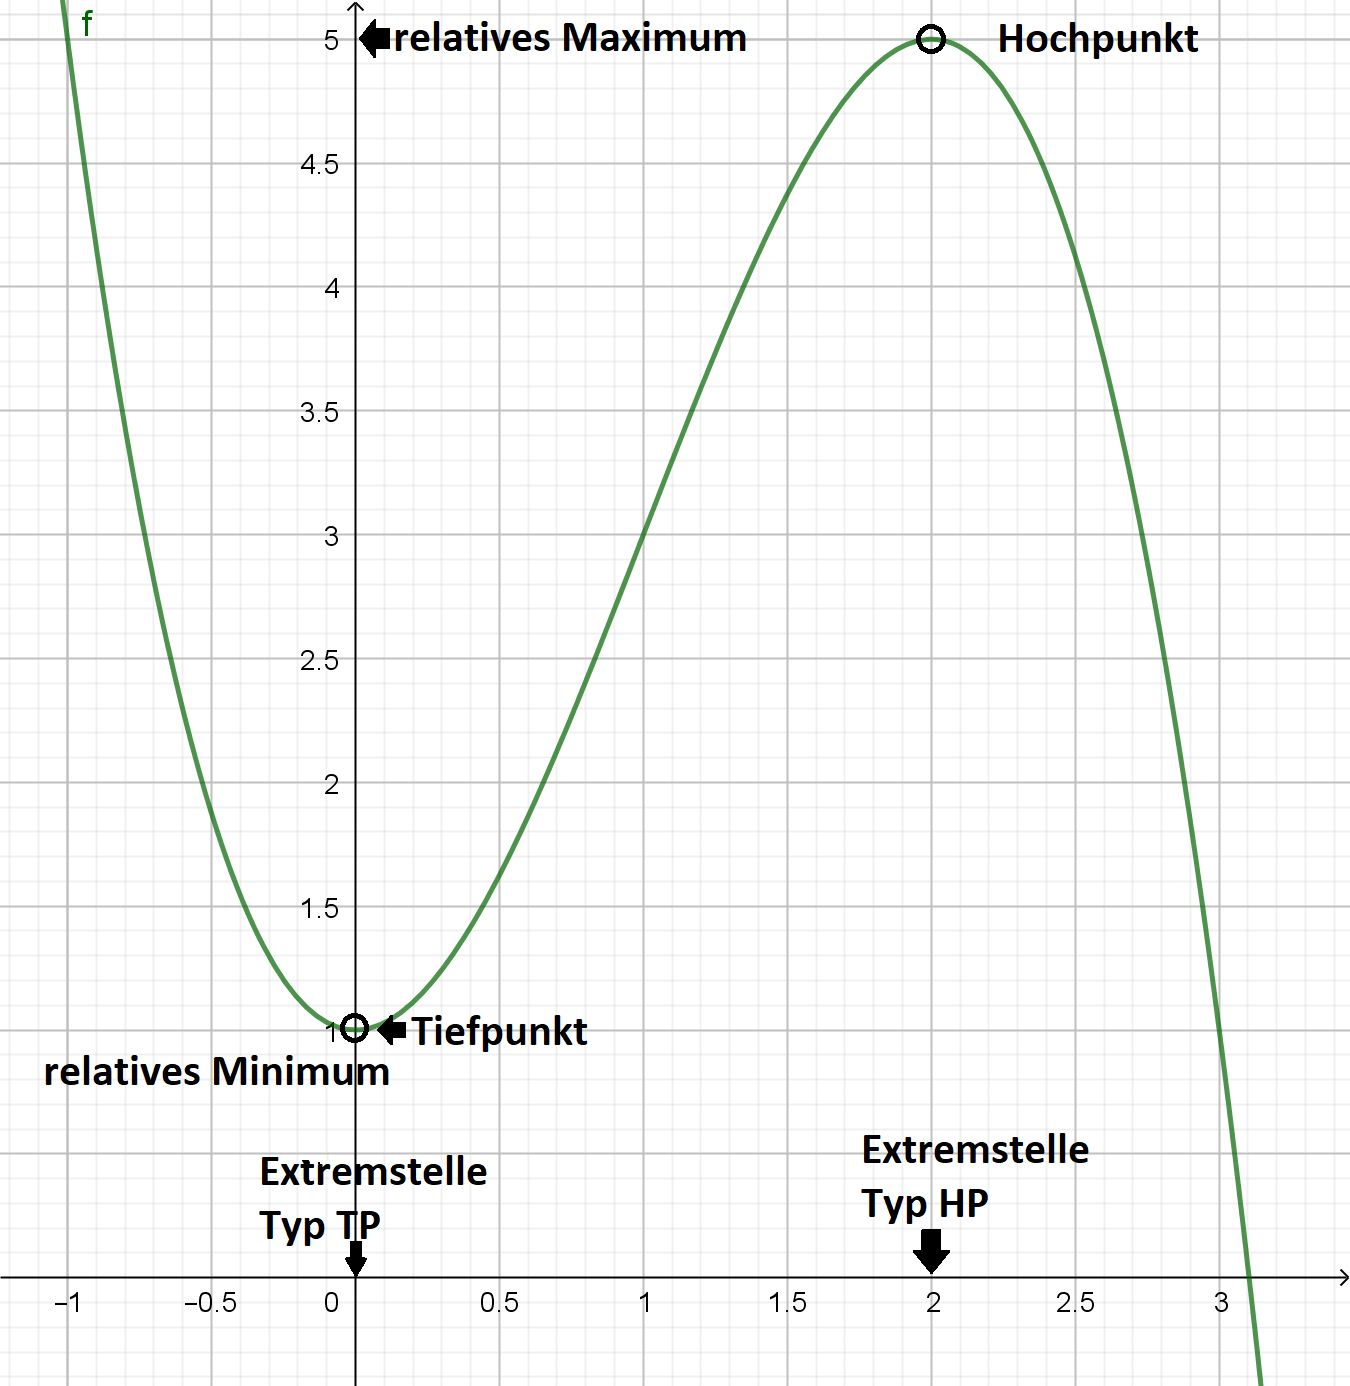
\includegraphics[width=0.49\textwidth]{../99_Bilder/EP.png}\\
		\par\bigskip\noindent
		Der Graph hat Extremstellen bei \(x_{TP} = 0\) und \(x_{HP} = 2\).\\
		Die dazugehörigen Punkte \textbf{Tiefpunkt (0|1)} und \textbf{Hochpunkt (2|5)}.\\
		Daraus können die relativen Minima bzw. Maxima ablesbar. So ergibt sich das \textbf{relative Minimum} bei \( y_{MIN} = 1\) und das \textbf{relative Maximum} bei \(y_{MAX} = 5\).
		\subsection*{Krümmungsverhalten und Wendestelle}
		Stellt man sich den Graphen als einen Berg vor, ist logisch, dass es ab der Extremstelle \(x_{TP} = 0\) aufwärts geht, man also ansteigt. Zunächst wird die Steigung immer größer, also steiler. Ab der Stelle \(x = 1\) steigt man zwar weiterhin an, aber die Intensität der Steigung wird weniger - also flacht der Berg langsam ab.\\
		Diesen Wechsel kann man mit dem \textbf{Krümmungsverhalten} beschreiben. Die Stelle, an der sich das Krümmungsverhalten änder, nennt man \textbf{\underline{Wendestelle}}. Der dazugehörige Punkt heißt \underline{Wendepunkt}.\\
		\par\bigskip\noindent
		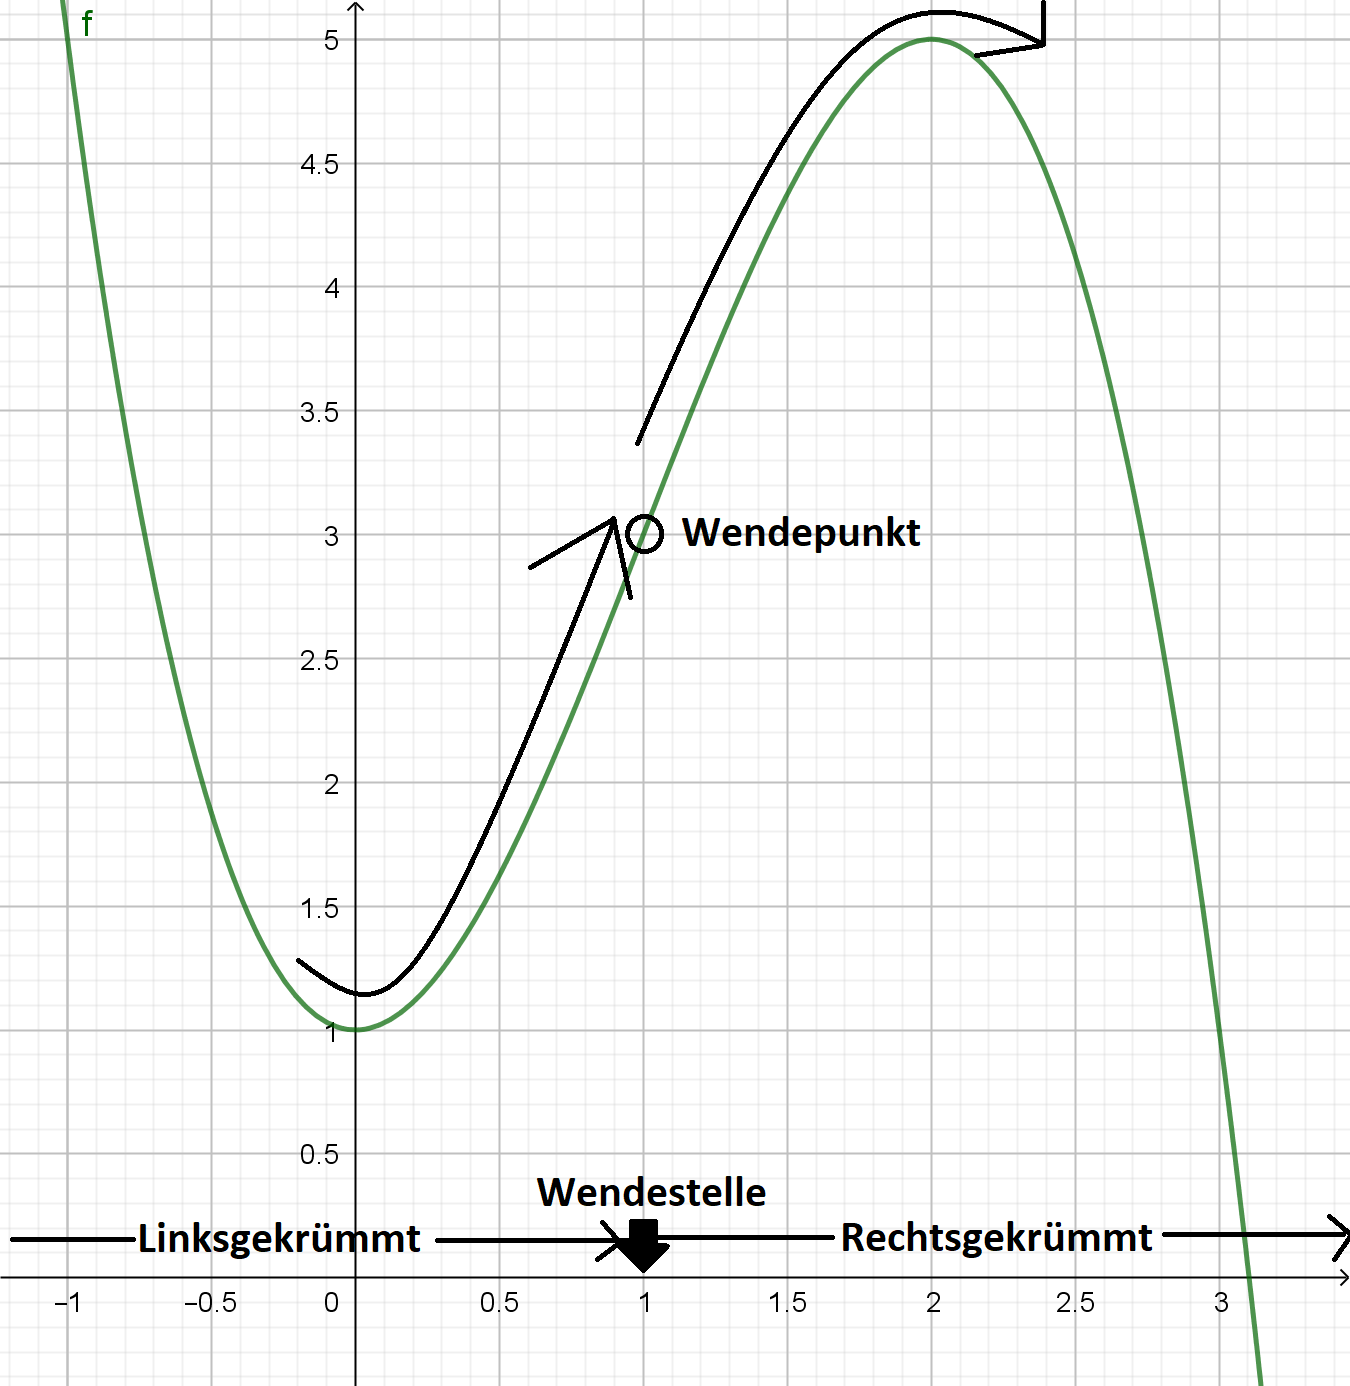
\includegraphics[width=0.49\textwidth]{../99_Bilder/WP.png}\\
		\par\bigskip\noindent
		\textit{Wichtig ist, dass das Krümmungsverhalten wie angegeben, \glqq{}links-\grqq{} bzw. \glqq{}rechtsgekrümmt\grqq{} nur korrekt ist, wenn man den Graph mit dem Auge entsprechend der Orientierung der x-Achse, also on positive x-Richtung, verfolgt.\\ Daher ist das Anbringen eines weiteren Pfeils links an der x-Achse strengstens untersagt.}
		\section{Funktionstypen}
		Es gibt verschiedene Arten von Funktionstypen. Diese werden in den nachfolgenden Abschnitten kurz erläutert.
		\subsection{Funktionstypen und ihre Prototypen}
		Die nachfolgende Tabelle gibt einen Überblick über diese. Zusätzlich werden die Prototypen der dazugehörigen Gleichungen angegeben, so dass Sie in Zukunft anhand des Funktionsterms den Funktionstypen erkennen können.\\
		\par\bigskip\noindent
		\begin{tabularx}{0.5\textwidth}{|X|X|}
			\hline
			\textbf{Funktionstyp} & \textbf{Prototyp der Gleichung}\\
			\hline
			Lineare Funktionen & \(y = m\cdot{}x + b\)\\
			\hline
			Quadratische Funktionen & \(y = a_2\cdot{}x^2 + a_1\cdot{}x + a_0\)\\
			\hline
			Ganzrationale Funktionen & \(y = a_n\cdot{}x^n + \ldots{} + a_2\cdot{}x^2 + a_1\cdot{}x + a_0\)\\
			\hline
			Exponential Funktionen & \(y = a\cdot{} b^x\)\\
			\hline
			Potenzfunktion & \(y = x^a\)\\
			& a ist eine rationale Zahl\\
			\hline
			Wurzelfunktion & \(y = \sqrt{x}\)\\
			\hline
			Gebrochen-rationale Funktionen & \(y = \frac{a_n\cdot{}x^n + \ldots{} + a_1\cdot{}x + a_0}{b_m\cdot{}x^m + \ldots{} + b_1\cdot{}x + b_0}\)\\
			\hline
		\end{tabularx}
		\subsection{Verkettete Funktionen}
		Es kann auch passieren, dass verschiedene Funktionstypen miteinander verkettet werden.\\
		So kann zum Beispiel eine \underline{Lineare Funktion} mit einer \underline{Potenzfunktion} verkettet werden: \(y = (x +5)^4\)
	\end{worksheet}
	\begin{worksheet}{Höhere Berufsfachschule IT-Systeme}{Grundstufe - Mathematik}{Arbeiten mit Funktionen}
		\setcounter{section}{0}
		\section{Spezialitäten und Tricks}
		Im Idealfall bereitet eine Funktionsgleichung sogut wie keine Probleme beim Zeichnen des Graphen. Die bekannte Wertetabelle liefert ausreichend viele Punkte, um einen ordentlichen Ausschnitt des Graphen zu zeichnen, aus dem die im Kapitel \glqq{}Grundlagen Funktionen\grqq{} angesprochenen Charakteristika des Graphen deutlich hervorgehen.\\
		\underline{Aber} es gibt auch Funktionstypen mit Besonderheiten. Nachfolgend werden einzelne Besonderheiten aufgeführt und wie sie damit umgehen können.
		\subsection{Besonderheit 1 - Außergewöhnliche Wertetabelle}
		Es kann passieren, dass die aufgestellte Wertetabelle es nicht ermöglicht einen wirklich plausiblen Graphen zu skizzieren.\\
		Bei der Funktion \(y = x^3-3x^2 + 2x\) sieht die Wertetabelle wie folgt aus:
		\begin{tabularx}{0.5\textwidth}{|l|l|l|l|l|l|}
			x & \(-1\) & \(0\) & \(1\) & \(2\) & \(3\)\\
			\hline
			y & \(-6\) & \(0\) & \(0\) & \(0\) & \(6\)
		\end{tabularx}
		Es ist unschwer erkennbar, dass das zugehörige Koordinatensystem so aussieht:\\
		\par\bigskip\noindent
		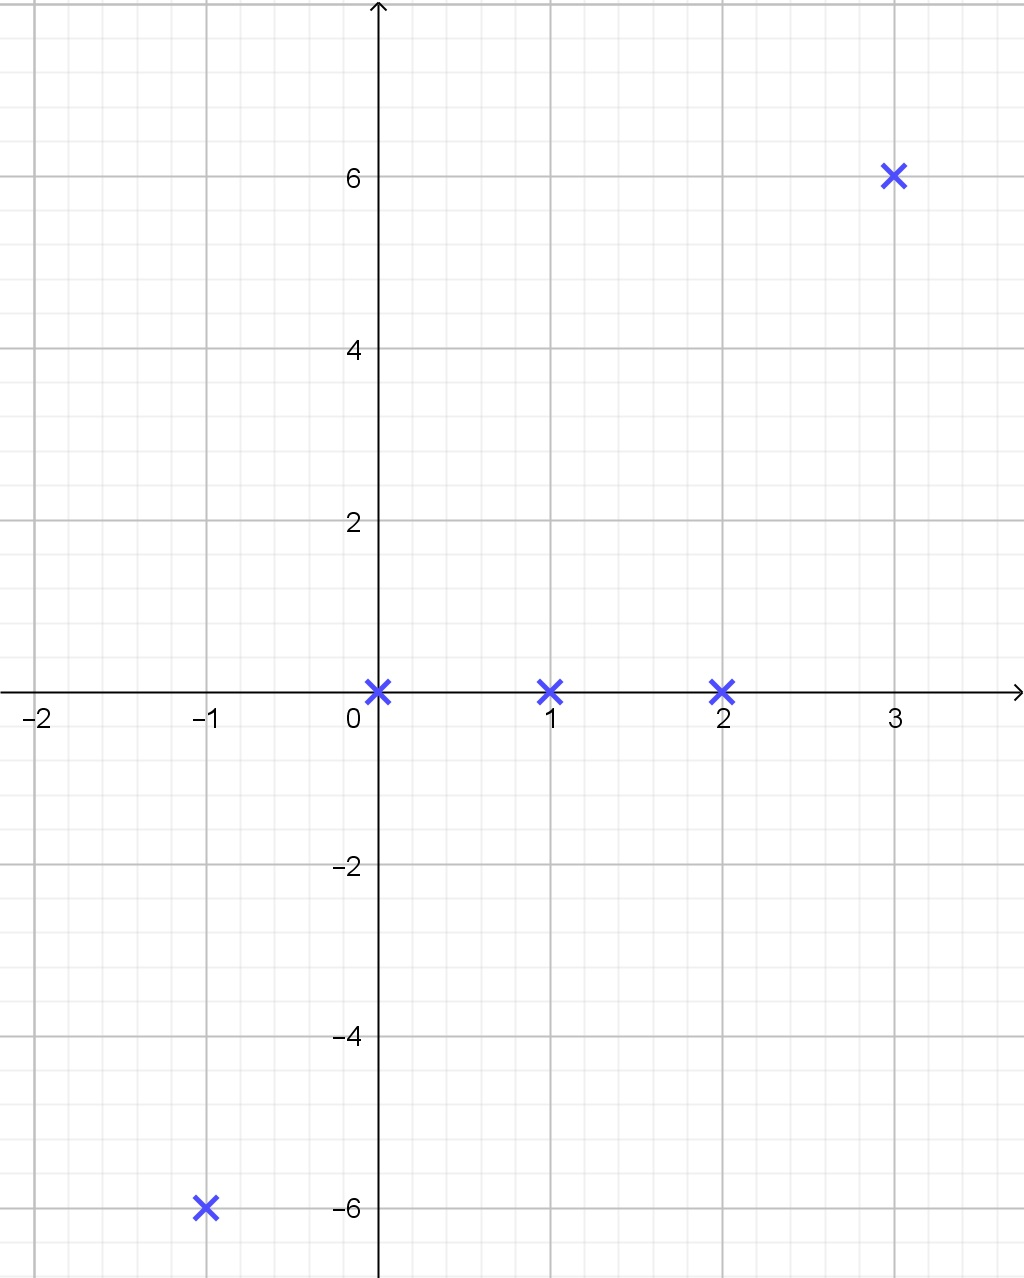
\includegraphics[width=0.49\textwidth]{../99_Bilder/b1Koord.jpg}\\
		\par\bigskip\noindent
		Hier kann es Helfen, wenn man die Wertetabelle verfeinert und so mehr Punkte zum eintragen erhält.\\
		\par\bigskip\noindent
		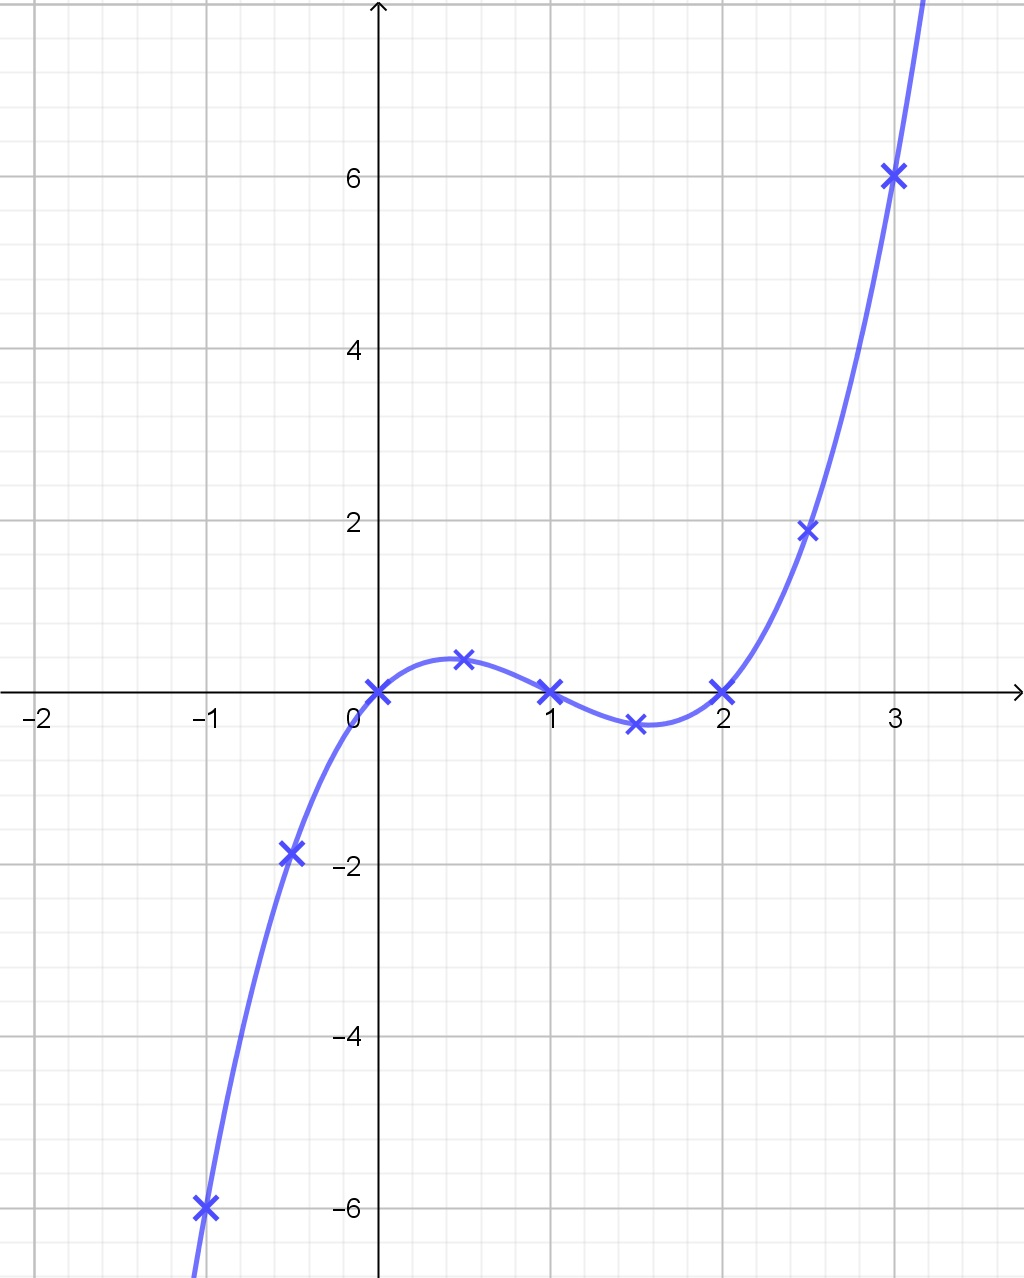
\includegraphics[width=0.49\textwidth]{../99_Bilder/b1Koord1.jpg}\\
		\subsection{Besonderheit 2 - Unklare Skalierung}
		Zwar haben wir eine Wertetabelle mit ausreichend vielen Wertepaaren, aber daraus ist nur schwer ersichtlich, wie die Skalierung der y-Achse zu wählen ist, um die Charakteristika zu verdeutlichen.\\
		\textbf{Beispiel: Bevölkerungswachstun Rheinland-Pfalz}\\
		\begin{tabularx}{0.49\textwidth}{|l|l|l|l|l|l|l|}
			\hline
			x & \(0\) & \(1\) & \(2\) & \(3\) & \(4\) & \(5\)\\
			\hline
			y & \(3555\) & \(3602\) & \(3550\) & \(3578\) & \(3629\) & \(3698\)\\
			\hline
		\end{tabularx}
		\par\bigskip\noindent
		\begin{tabularx}{0.5\textwidth}{l|l|l|l|}
			\cline{2-4}
			& \(6\) & \(7\) & \(8\)\\
			\cline{2-4}
			& \(3773\) & \(3848\) & \(3913\)\\
			\cline{2-4}
		\end{tabularx}
		\par\bigskip\noindent
		Natürlich müssen auf der x-Achse die Werte 0 bis 8 abgetragen werden. Die Skalierung kann hier wie üblich gewählt werden.\\
		Wie aber sieht es auf der y-Achse aus? Hier sollen wir auf 10 cm Werte bis \(4000\) abtragen. Eine Möglichkeit wäre es, je \textbf{1 cm} immer \(400\) abzutragen.\\
		\par\bigskip\noindent
		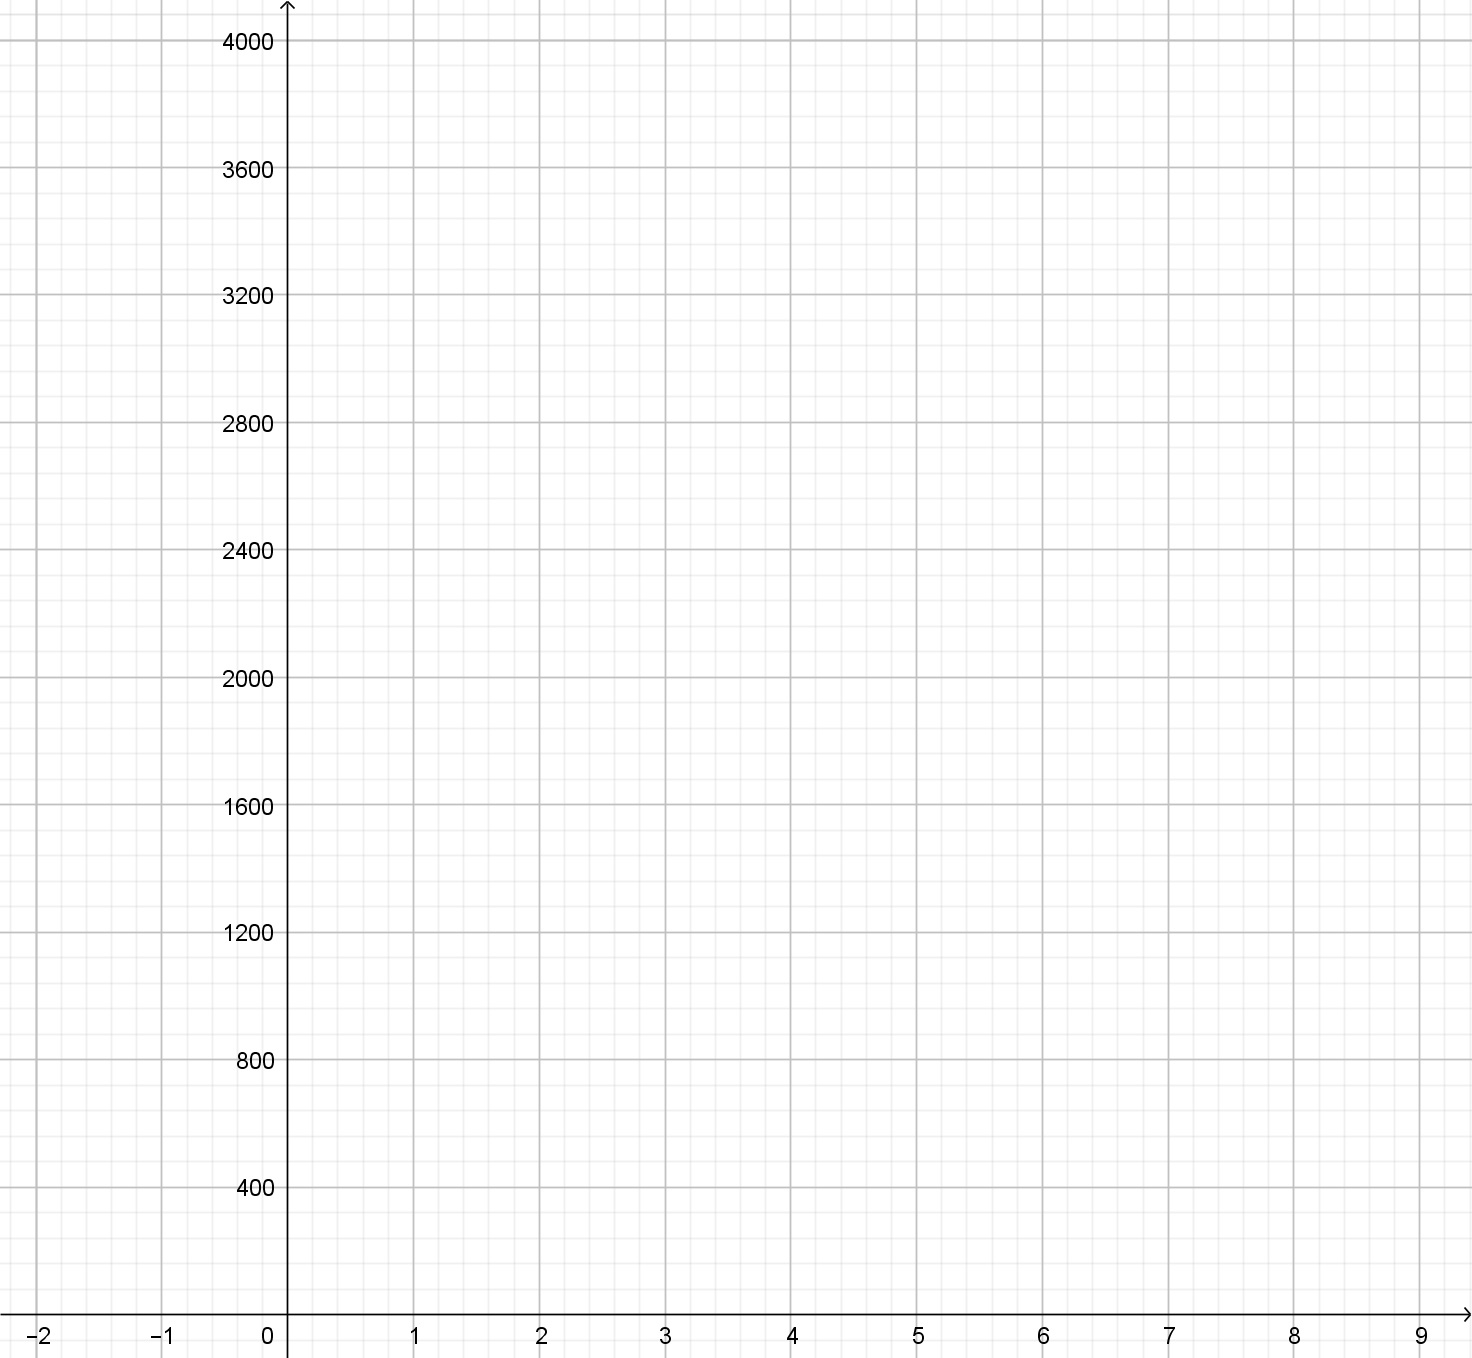
\includegraphics[width=0.49\textwidth]{../99_Bilder/b2Koord.jpg}\\
		\par\bigskip\noindent
		Aus der Wertetabelle ist aber erkennbar, dass unser niedrigster y-Wert \(3550\) ist, wir benötigen also die Werte 0 bis \(3549\) nicht. Damit eröffnet sich eine andere Möglichkeit.\\
		Wir beginnen im Ursprung mit dem y-Wert \(3500\) und erhöhen diesen je \textbf{1 cm} um 50.\\
		\par\bigskip\noindent
		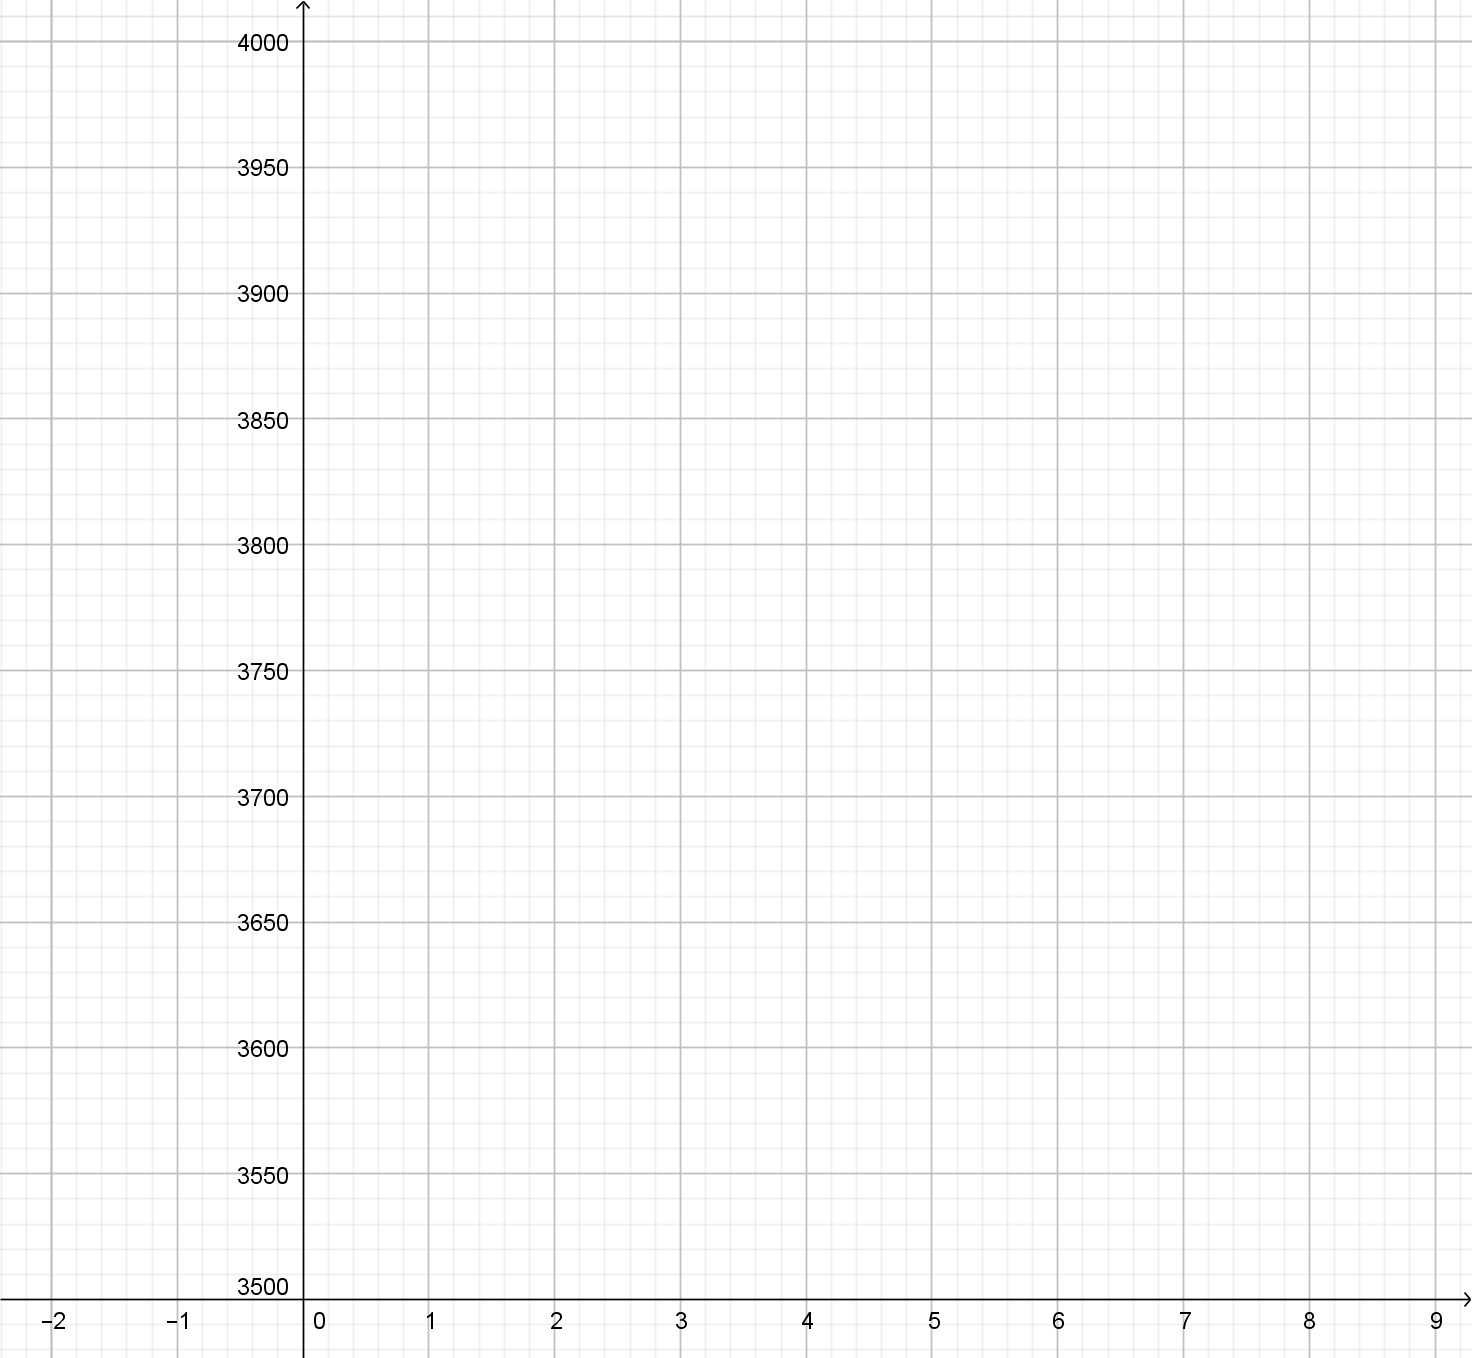
\includegraphics[width=0.49\textwidth]{../99_Bilder/b2Koord1.jpg}\\
		\par\bigskip\noindent
		\textit{\textbf{Vorsicht:} Wurde die Einheit für eine Achse festgelegt, so gilt diese für die gesamte Achse und \underline{darf nicht} geändert werden.}
	\end{worksheet}
\end{document}